\chapter{Egyensúlyozás}\label{ch:EGYENSULY}
\begin{osszefoglal}
E fejezet célja, hogy bemutassa a PID szabályzó algoritmus működését. E mellet sorkelűr az egyensúlyozás működésének leírására, valamint hogy miként lehet felhasználni ez esetbe a PID szabályzó algoritmust.
\end{osszefoglal}

\section{PID szabályzó algoritmus}\label{sec:EGYENSULY:pid}
A PID \texttt{(Proportional Integral Derivate)} elterjedt algoritmus az ipari szabályzó körökben köszönhetően a viszonylag egyszerű félépítéséért és a könnyen kezelhetőségéért. Számos felhasználási lehetősége van, ilyenek a nyomás, hőmérséklet, sebesség szabályozás.

A PID, mint a nevéből is látható három tagból tevődik össze: P \texttt{(Proportional)} proporcinális tag, I \texttt{(Integral)} a hibák integrált tagja és a D \texttt{(Derivate)} a hibák időbeli változásának derivált tagja. Több változata is van, azok az esetek mikor nem valósulnak meg az előbb felsoroltak mindegyike, ilyenkor beszélünk P, PI, PD szabályokról.

PID szabályzó matematikai képlete: $$u(t)=K_{P}e(t)+K_{I}\int e(t)dt+K_{D}\frac{d}{dt}e(t),$$ ahol bemeneti hiba jelöle az e(t), u(t) a kimenet. A $K_{P}, K_{I}, K_{D}$ rendre a proporcinális, integrált és a derivált súlyát határozzák meg.

Esetünkben a P az aktuális hiba, I a hibák összességének integráltja, D az aktuális és az előző hiba időbeli változásának deriváltja. A tagok súlyát meghatározó konstansok jelentős befolyással vannak a kimenetre. 

A $K_{P}$ befolyásolja a szabályzó érzékenységét, instabilitást okozhat. A magas erősítés, amely nagy oszcillációt idéz elő, ellentétben áll az alacsony erősítéssel, hiszen az utóbbi kicsi oszcillációt idéz elő. Ezen estekben a robot elveszti az egyensúlyi állapotát. 

A $K_{I}$ erősítő esetén figyelembe kell venni, hogy az integrált tag folytonosan nő és a túl nagy érték túllendülést eredményez. 

A $K_{D}$ a hiba változásának mértékét határozza meg. Amennyiben az aktuális és előző hiba közti különbség nagy, hirtelen változást idéz elő a szabályzó kimenetén. A derivált szerepe, hogy csökkentse a kimenet hirtelen változását, megakadályozva a hirtelen sebesség növekedést. Magas erősítés okozhat instabilitási problémákat.

A \ref{pidFig} ábrán látható a PID szabályzó tagjainak változása. Az $I$ tag domináns a $P$ illetve $D$ tagokkal szemben, látható hogy az integrált tag folyamatosan növekszik. Annak érdekében, hogy túllendülést okozzon az integrált, a derivált tagnak kell ellensúlyozza.

A $P$ tag az előbb említett két tag nagysága között változik. E tag esetén a túl nagy oszcilláció azt idézné elő, hogy a robot hirtelen reagálna az eldőlésre ezért átlendítené ellentétes irányba annyira, hogy eldőlne. Ezzel ellentétbe, a kisebb oszcilláció hatására megfigyelhető lenne a roboton, hogy a vártnál később reagál az egyensúly korrigálására és ebben az esetben is eldőlne.

\begin{figure}[!htb]
	\begin{center}
		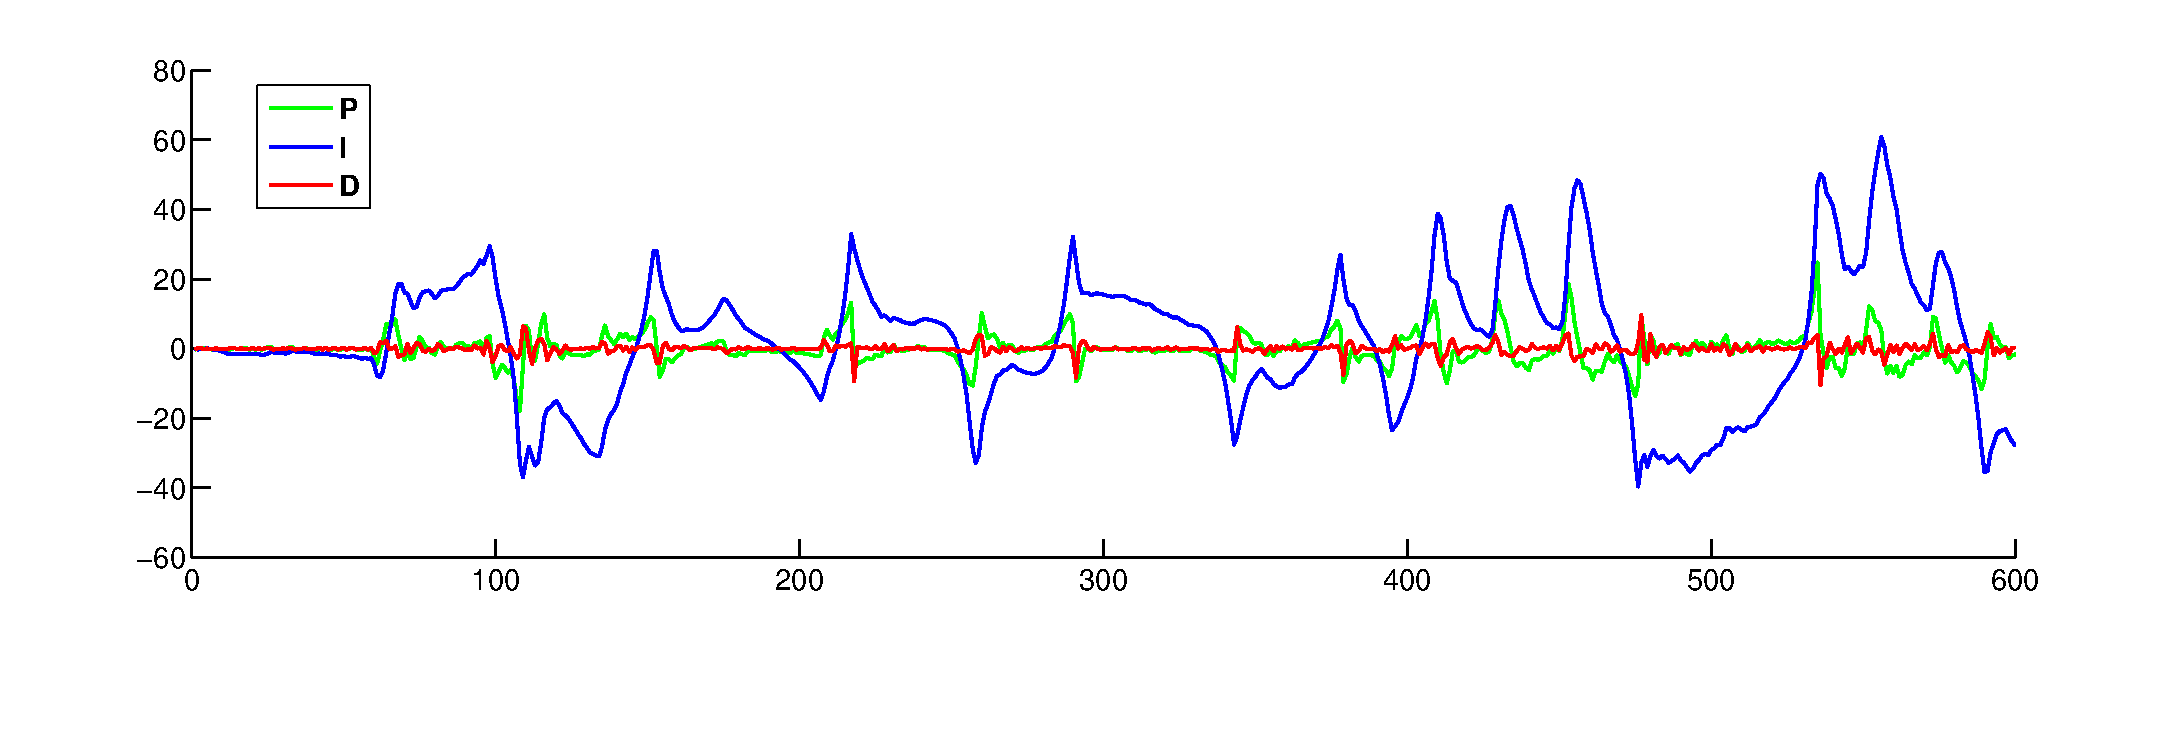
\includegraphics[width=1.0\linewidth]{images/pid.eps}
	\end{center}
	\caption{PID tagjai egyensúlyi állapotban}
	\label{pidFig}
\end{figure}
